\documentclass[letterpaper,10pt,draftclsnofoot,onecolumn,compsoc]{IEEEtran}
\usepackage{graphicx}
\usepackage{amssymb}
\usepackage{amsmath}
\usepackage{array}
\usepackage{amsthm}
\usepackage{listings}
\usepackage{alltt}
\usepackage{float}
\usepackage{color}
\usepackage{url}
\usepackage{setspace}
\usepackage{balance}
\usepackage{enumitem}
\usepackage{pstricks, pst-node}
\usepackage{inputenc}
\usepackage[margin=.75in]{geometry}

\newcommand{\subparagraph}{}
\usepackage{titlesec}
\setlength{\abovecaptionskip}{2pt}
\setlength{\belowcaptionskip}{0pt}
\usepackage{fancyhdr}
\usepackage{hyperref}
\usepackage{tocloft}

\lstset{language=HTML,
        showstringspaces=false}

%hide toc subsubsections
\setcounter{tocdepth}{2}
\setlength{\parindent}{.0in}

%toc formatting for IEEE 830-1998 standards
\renewcommand{\cftsecleader}{\cftdotfill{\cftdotsep}{\vspace{.25cm}}}
\renewcommand{\cftsecfont}{\normalfont}
\renewcommand{\cftsecpagefont}{\normalfont}
\renewcommand{\cftsecaftersnum}{.}

%bottom right page numbers
\fancyhf{}
\renewcommand{\headrulewidth}{0pt}
\rfoot{\thepage}
\pagestyle{fancy}

%formatting specific IEEE 830-1998 Section headings
\titleformat{\section}[block]
  {\fontsize{12}{10}\bfseries\sffamily}
  {\thesection.}
  {1em}
  {\vspace{.25cm}}
\titleformat{\subsection}[block]
  {\fontsize{10}{10}\bfseries\sffamily}
  {\thesubsection}
  {1em}
  {\vspace{.25cm}}
\titleformat{\subsubsection}[block]
  {\fontsize{10}{10}\bfseries\sffamily}
  {\thesubsubsection}
  {1em}
  {\vspace{.25cm}}
\titleformat{\subsubsubsection}[block]
  {\fontsize{10}{10}\bfseries\sffamily}
  {\thesubsubsection}
  {1em}
  {\vspace{.25cm}}
  
\newcommand{\cred}[1]{{\color{red}#1}}
\newcommand{\cblue}[1]{{\color{blue}#1}}

\def\name{Charles Siebert, Branden Berlin, Yipeng "Roger" Song}

%% The following metadata will show up in the PDF properties
\hypersetup{
  urlcolor = black,
  pdfauthor = {\name},
  pdfkeywords = {cs461 ``Senior Capstone - Fall 2016'' capstone},
  pdftitle = {CS 461 Requirements Document},
  pdfsubject = {Capstone Requirements Document},
  pdfpagemode = UseNone
}

\begin{document}
\begin{titlepage}
\centering
\vspace*{6cm}
{\scshape\LARGE \begin{singlespace}Optimizing Virtual Reality and Augmented Reality Performance on Mobile Web Applications \\ \end{singlespace} Design Document } \\
	{\scshape\Large CS461 - Fall 2016 \par}
	\vspace{.5cm}
	\name \par
    {\large \today \par} 
	\vspace*{1cm}
	
\begin{abstract}
The technology of Virtual Reality (VR) currently is not cost effective to today's market, as the cost of high-end setups required makes it difficult to afford. Browser developers are focusing primarily on expensive high-end high-performance hardware over mobile devices for Augmented Reality (AR) or Virtual Reality (VR) on the web. Doing AR/VR on the mobile web allows more developers to enter the field and deliver to more customers. To accomplish this, we are working on a project called �Mobile AR/VR Performance�, which focuses on researching to profile and identify performance bottlenecks in 3D web content on mobile devices. We will file issues in the open source projects for Chrome, Firefox through A-Frame and Three.js to determine and identify those bottlenecks. We hope to accomplish this by reporting the challenges and opportunities for performance VR/AR applications, and write a blog post detailing the project results and their best-practices.
\end{abstract}

\end{titlepage}

\newpage

\tableofcontents

%removes page number on table of contents
\thispagestyle{empty}

\newpage

\section{Introduction}
\begin{singlespace}


\par Our project "Optimizing Virtual Reality and Augmented Reality Performance on Mobile Web Applications," nicknamed "OVRAR" is the development of a VR application and analyzing the performance based on the restrictions of using it in a mobile environment with the same devices. Using the data we collect from the application, we can determine specific bottlenecks and performance issues that may be incurred on the device based on different test implementations. This design document is the road map of our project for the rest of the year. We will follow the time line which has been discussed in this document strictly to keep us on the right track. Though little things may change in terms of detail, but the big picture will still be relevant. In this document, we will write up the design of nine pieces that have been discussed from the technology review. The design for each piece will include: describing design components and steps, creating and formatting a glossary; integrating multiple descriptions of design into a full document, referring to past learning (software engineering experience), and identifying appropriate language to fit genre (research project or product development project).

\subsection{Scope}


Optimizing VR and AR for Mobile Web Apps is to determine Virtual Reality (VR) and Augmented Reality (AR) bottlenecks that exist in mobile devices within the A-Frame framework. The bottlenecks can be caused from either unoptimized development of software, underpowered or unoptimized hardware found in existing devices, or potential bugs or limitations found within the framework itself. The software itself, which is developed on A-Frame, will generate multiple scenes where it will test the graphical capabilities of the hardware within the mobile devices, the types of different implementations of certain scenes, and determine areas of optimization through these multiple scenes. The software will be used to create a report that will analyze the information collected about processing power, frame rates, battery usage, and the limitations of the framework to determine the best practices for implementing more graphically intensive programs on A-Frame. \\


Developers other than us will use the information in the report to determine the best way to approach at designing their programs, as the software we create will only serve as test cases and stress testing for mobile devices to collect this information. 

\subsection{Purpose}
The purpose of this project is to determine areas of development within A-Frame where practices will be best used, as they will least be likely to impede on bottle necking either the software or hardware whe n optimizing the software for performance. This project is focused towards the advancement of an open-source, developing web framework, and the developers making their own products with A-Frame and for mobile devices. The developers will be using our project research as a means to avoid these bottlenecks in this evolving environment.
\end{singlespace}

\newpage

\begin{thebibliography}{9}

\bibitem{android} 
Vogella. 
\textit{Android Application Performance Profiling through Android SDK}. 
\\\texttt{http://www.vogella.com/tutorials/AndroidTools/article.html}

\bibitem{firefox} 
Mozilla Developer Network.
\textit{Firefox Developer Tools}.
\\\texttt{https://developer.mozilla.org/en-US/docs/Tools}

\bibitem{chrome} 
Google Chrome DevTools. 
\textit{Chrome DevTools}.
\\\texttt{https://developers.google.com/web/tools/chrome-devtools/}

\bibitem{phonespec}
GSM Arena.
\textit{Phone Specifications}
\\\texttt{http://www.gsmarena.com/}

\bibitem{aframe} 
A-Frame. 
\textit{Building a Basic Scene in A-Frame}.
\\\texttt{https://aframe.io/docs/0.2.0/guide/building-a-basic-scene.html}

\end{thebibliography}

\section{Glossary}
\begin{singlespace}
\begin{enumerate}[labelsep=2em,leftmargin=.5in]
    {\item \bfseries Virtual Reality (VR): } Computer generated three-dimensional environment that immerses the user into the environment using special equipment or implementation techniques. \vspace{.1cm}
    {\item \bfseries Augmented Reality (AR): } Provides a composite view to the user based on computer generated environments super-imposed onto the view of the real world. \vspace{.1cm}
    {\item \bfseries Operating System (OS): } Software that supports an interface to support computer's basic functions, such as process scheduling, executing tasks, and allowing user interface. Specifically this project is in regards to Android OS. \vspace{.1cm}
    {\item \bfseries Web Framework: } A software framework that is designed to support the development of web applications including web services, web resources and web APIs. \vspace{.1cm}
    {\item \bfseries A-Frame: } A-Frame is an open-source WebVR framework for creating virtual reality (VR) experiences with HTML with the use of the Three.js framework.\vspace{.1cm}
    {\item \bfseries Three.js: } JavaScript framework that allows accessible development WebGL applications. \vspace{.1cm}
    {\item \bfseries WebGL: } JavaScript API that allows for rendering interactive 3D and 2D computer graphics within any compatible web browser without the use of plug-ins. \vspace{.1cm}
    {\item \bfseries Viewport: } A viewport is a viewing region in computer graphics. This region is defined in the software to allow for viewing the drawing of objects. This viewport is typically bounded by a window or by the full screen of the mobile device. \vspace{.1cm}
    {\item \bfseries Local Web Server: } A web server for hosting web page content to allow access on local networks, without having to go out into the internet to access the information. \vspace{.1cm}
    {\item \bfseries Hosted Web Server: } A server that is hosted externally on the internet, where it holds and displays the web information, needing to go out to the internet, and back again to receive the proper information. \vspace{.1cm}
    {\item \bfseries Implementation Languages: } a formal computer language or constructed language designed to communicate instructions to a machine, particularly a computer. i.e. HTML, JavaScript, C, C++, etc. \vspace{.1cm}
    {\item \bfseries Mobile Devices: } A device that is able to be held and portable by a user, typically a smart phone or table.t\vspace{.1cm}
    {\item \bfseries Rendering: } Part of the graphical process that draws everything into the "view's" scene. This includes textures, animations, objects, surface information, etc. \vspace{.1cm}
    {\item \bfseries Bottleneck: } An effect impeding on the rendering process, which occurs between the hardware and software aspects. \vspace{.1cm}
    {\item \bfseries Optimize: } Process of making something as fully functional or effective as possible, including the types of limitations that occur in the environment. \vspace{.1cm}
    {\item \bfseries Performance: } The process of how well the software handles the action or function of the software.
    {\item \bfseries Software Bug: } An error, flaw, failure or fault in the system that causes it to produce an incorrect or unexpected result, or to behave in unintended ways. \vspace{.1cm}
    %{\item \bfseries [word]: } Something \vspace{.1cm}
\end{enumerate}

\newpage

\section{Design Concerns}
The design stakeholder for this project is Mozilla, and they tasked us to research areas of implementation on a framework called A-Frame. The design concerns they have for us to finish the project based on their requirements depend on the different ways of our program's implementation, rendering the scenes properly through a mobile device, capturing meaningful data from the mobile device, importing the information to be readable, and drawing conclusions based on the information attained. Specifically in terms of our software, the program needs multiple different scenes to be drawn in order to create a standard of testing in order to determine areas of bottlenecks or optimization issues that occur within the scene. These scenes need to be rendered in different ways in order to collect information that is meaningful to determine the specific areas that do have issues. The issues can range from rendering issues on the mobile device, Mozilla Firefox, Google Chrome, A-Frame framework, Three.js framework, or even with Android itself. The purpose of the project itself is to draw conclusions from this information in order to form a report at the end of the project that will detail how these bottlenecks exist, and how to avoid it. The rendering of scenes also have to fit within a set of constraints imposed by the mobile device itself.

\section{Design Constraints}
As the purpose of the project is to optimize and find bottleneck issues within the different levels of the frameworks, constraints of the software only exist based on the physical capabilities of the mobile device itself. We established guidelines that determine whether or not we fit within our constraints during our implementation. Based on these constraints, if we exceed them, then our job to optimize performance and find bottlenecks will ultimately not be accomplished.\smallskip

\begin{enumerate}[labelsep=2em,leftmargin=.5in]
    \item The software will be ran and tested on the mobile device used for this project, the Nexus 5X.
    \item Response time from user interaction to software processing information to be .1 second (about 3 frames of input delay).
    \item The software will display 30 Frames Per Second (FPS) to the phone through the viewport.
    \item The software will not exceed the amount of on-board RAM (2GB) during the time of drawing and texturing the scenes.
    \item The processors will not exceed the maximum usage (100\%) while the device is rendering the scene.
    \begin{enumerate}[leftmargin=*,labelindent=0pt]
        \item Due to possible hardware bottlenecks, if the processor usage does exceed 100\%, it will still allow the viewing of the scene with the aforementioned requirements.
    \end{enumerate}
    \item The software will not exceed excessive battery usage. The Nexus 5X has a total capacity of 2700 mAh.
    \begin{enumerate}[leftmargin=*,labelindent=0pt]
        \item Excessive battery usage will be measured how much battery capacity is used per hour.
        \item The battery should at the least last three hours on a full charge while undergoing the tests of this program.
    \end{enumerate}
    \item The software will not produce excessive heat through hardware being stressed by the software.
    \begin{enumerate}[leftmargin=*,labelindent=0pt]
        \item Excessive heat is defined to be a high enough temperature to trigger the phone's internal underclocking feature to reduce the temperature.
        \item Documentation, at this time, cannot be found at what temperature this occurs, but the temperature of the phone and the components will be tracked and documented if it causes the aforementioned requirements to not be met.
    \end{enumerate}
\end{enumerate}

\section{Design Viewpoints}
The design viewpoints for this project will address the concerns brought up by our client, and provide insight to the interactions between the different entities involved in completing this project. The viewpoints are to provide a certain perspective at each component level within the entities. For example, we will be discussing the relationship between capturing the data from the phone while it is rendering scenes and how that relationship exists when storing that information to be parsed into readable and understandable information that can be digested. The purpose of this is to break down the components to determine the analysis techniques we will be using throughout this project and the hueristic guildelines to assist in evaluating and determining the tool and process we will use to accomplish a task. For this document to be complete, each view should address the concerns listed in Section 3.

\subsection{Context (Development) Viewpoint}
This viewpoint is special in our sense as a research project, where documentation and proper development is needed. Our project will undergo many revisions due to the nature of our testing, reiteration and retesting. The concerns this brings up is being able to go back to older revisions, and determine the kind of implementations are causing certain slow-downs. This brings up a need to have proper version controlling, documentation and development tools. In order to have proper version control and documentation, we decided documenting our findings and information to be best in a parsable format (such as \LaTeX), and avoid binary files, as we will be using Github as our form of version control.

\subsubsection{Development Tools View (Roger)}
In order to develop a software project as a group, one biggest point is to choose the right development tool. In this project, we are going to use Visual Studio as the development tool because Visual Studio is often used to develop computer programs for Microsoft Windows, as well as web sites, web applications and web services which our project is mainly focus on. \\

The biggest reason that we choose Visual Studio to be our development tour is that Visual Studio offers a comprehensive development environment to help Web developers build standards-based Web applications and services. It improves productivity by allowing users to rapidly develop, test and deploy Web solutions. Additionally, Visual Studio offers a free version aimed at Web developers. With Visual Web Developer Express, you get a full featured web development environment for working with ASP.NET, JavaScript and Web standards. \\

The goal of Visual Studio is to provide rich development tools to all developers globally on any platform. Development teams will be able to develop software for Web, mobile, server and desktop with Visual Studio. Also, it also has an online version  Visual Studio Online, which is a set of tools that makes it much easier for continuous integration across different platforms. \\

\subsubsection{Version Control and Documentation View}
Our deliverable product for this project will be a report detailing the results we've found through our sets of test cases, and so having proper version control and documentation is a key thing to have for this project. We have a need to be able to have information readily accessible to us for when we are dealing with multiple test cases, to be able to review previous results and data to be able to determine the cause of possible bottlenecks that occur in real time. We need to be able to reference our findings, import and export the data in a fashion that would not mess with the formatting of our documentation and handle imported into our choice of version control without issues. \\

LaTeX is a mark-up language, similar to HTML. As a word processor, it breaks down the formatting based on the packages included into the file, and the defined parameters allow uniform formatting in all specifically defined areas. Even graphics will be easily imported into the document, as tools such as PSTricks allow the rendering of the images based on a few function calls in the document, and when compiled it will generate the file properly. This fits in the scope for our project as it will fit within the use of our Github version control, and will allow us to see the changes made to the document and view them in real time. Having us to see the line changes specifically to the conclusions we make, on the particular implementations we are testing, allows us to easily compare and contrast the changes we made. This helps determine what areas caused good optimization, or bad areas of bottlenecks within the system. It's also very trivial to add special tables of data or analytical images as it is just a file with marked up text where formatting is already predefined.\\

\subsection{Composition Viewpoint}
For the composition viewpoint, the design concerns that is addressed in this is the concern of composition of A-Frame with the use of Three.js framework, which utilizes WebGL in order to render the scenes through the browser. Based on these concerns, we have to determine a way to render the scene through this composition. Since A-Frame is built off of HTML language, it makes use of calling JavaScript functions that are included, which will handle the entire scene generation through Three.js API calls to use WebGL to use the proper function calls to generate the objects.

\subsection{Language Tools View (Roger)}
An implementation language is a formal computer language or constructed language designed to communicate instructions to a machine, particularly a computer. Understanding difference(s) between programming languages is crucial. If wrong language is chosen for a project, it will take a lot of time and efforts to change the course and re-implement the project or its part in different language. For our project, since we are going to test the performance of web app through A-frame, which is a Web framework, so we should choose from the languages that are specific to web development. \\

As this project serves as to be used as research, correctness will be based off of how well we can push the boundaries of our software, based on the performance the hardware can provide. Therefore, we need to collect the information in different types of implementations between scenes the program generates, so we should be able to understand and write some test scripts. \\

HTML, stands for Hyper Text Markup Language, is the standard markup language for creating Web pages. It describes the structure of Web pages using markup, and its elements are the building blocks of HTML pages which are represented by tags. HTML tags label pieces of content such as "heading", "paragraph", "table", and so on. Browsers do not display the HTML tags, but use them to render the content of the page. HTML is easy enough to write, Much of the code can be customized by someone who knows proper HTML formatting. HTML also allows the use of templates, which makes designing a web page easily. \\

Programs written in JavaScript run in the web browser itself, so if the website has a JavaScript program, the program will be automatically fetched by your visitor's browser and executed on his/her computer. Therefore, JavaScript is very fast because any code functions can be run immediately instead of having to contact the server and wait for an answer. Plus, JavaScript is relatively simple to learn and implement, and it plays nicely with other languages and can be used in a huge variety of applications. Additionally, being client-side reduces the demand on the website server. \\

As discussed above, We are going to use HTML, and JavaScript simultaneously as language tools, as both of them are very crucial to our project. We need these languages in order to find the bottlenecks, where the optimization needs to be done. More specifically, we are going to implement test scripts, such as stress-testing, to help optimize the performance of the web app as long as we find some bugs. \\

\subsection{Logical Viewpoint}
In building the implementation, we will have to find of ways to stress the system and resources we have available. The concern is finding areas of implementation that actually cause issues with rendering, so we have to understand all the ways in how objects are rendered within the system, and what we can do to manipulate the objects to strain the system. With us needing to address the bottlenecks and optimization issues found in the web browsers, we need different ways to generate objects, and A-Frame allows for just that. While the following examples are simple to implement, they offer ways, in terms of big numbers, already to stress the system. When generating large amounts of objects, drastically increases the resources used by the system; large quality textures, animations, and redrawing the objects constantly can already easily bring the phone resources to our defined constraints.

\subsubsection{Create Scenes View (Roger)}
A-Frame is an open-source WebVR framework for creating virtual reality (VR) experiences with HTML with the use of the Three.js framework. As the purpose of this project is to determine areas of development within A-Frame, the first thing we need to know is how to create scenes using A-Frame. Primitives are the basic building blocks of A-Frame with familiar HTML syntax. A-Frame is bundled with a handful of primitives for common use cases such as backgrounds, colors, images, meshes, models, and videos. Following are the 4 most commonly used skills when creating scenes. After we get familiar with these, then we are able to research on things like what if binding a texture to 10,000 objects, how will these things affect the performance of the real program \cite{aframe}.

\subsubsection{Adding a Box}
We will get to know how A-Frame works by creating adding a box, which is the simplest scene would contain. 
\begin{figure}[H]
\caption{Adding a box}
\begin{lstlisting}
<a-scene>
    <a-box color="#6173F4" width="4" height="10" depth="2"></a-box>
</a-scene>
\end{lstlisting} 
\end{figure}

Just like with regular HTML elements, each attribute of the entity maps to one value. We can define a color, width, height, and depth of "a-box".
Once we open up our scene, the default control setup allows us to look and walk around. To look around, we can drag the mouse or just look around with a mobile device or a Rift. To walk around, we can use the WASD keys. 

\subsubsection{Transforming a Box}
As we learned, the basic distance unit in A-Frame is defined in meters. When designing a scene for virtual reality, it is important to consider the real world scale of the objects we create. For example, a box with height="100" may look ordinary on our computer screens, but in virtual reality it will look like a massive 100-meter tall monolith. To translate, rotate, and scale the box, we can plug in the position, rotation, and scale components. The example below (assuming we are positioned on the origin looking down the negative Z-axis) will translate the box left/up/back, rotate the box to the right, stretches the box left-and-right and back-and-front, and shrinks the box up-and-down: 

\begin{figure}[H]
\caption{Transforming a box}
\begin{lstlisting}
<a-scene>
    <a-box color="#6173F4" width="4" height="10" depth="2"
        position="-10 2 -5" rotation="0 0 45" scale="2 0.5 3"></a-box>
</a-scene>
\end{lstlisting} 
\end{figure}

\subsubsection{Applying a Texture to the Box}
The box doesn�t have to be just a flat color. We can wrap a texture around the box with an image or video using "src". To cache the texture and have the scene wait for it to load before rendering, we can move the texture into the asset management system. We define it as an "img" tag, give it an ID, and point to it using a selector:
\begin{figure}[H]
\caption{Applying a Texture to the box}
\begin{lstlisting}
<a-scene>
   <a-assets>
        <img id="texture" src="texture.png">
    </a-assets>
    <a-box color="#FFF" width="4" height="10" depth="2"
        position="-10 2 -5" rotation="0 0 45" scale="2 0.5 3"
        src="#texture"></a-box>
</a-scene>
\end{lstlisting} 
\end{figure}

\subsubsection{Animating the Box}
We can also add an animation to the box. An animation is defined by placing an "a-animation" tag as a child of the entity to animate.
\begin{figure}[H]
\caption{Animating the box}
\begin{lstlisting}
<a-scene>
   <a-assets>
        <img id="texture" src="texture.png">
   </a-assets>
   <a-box color="#FFF" width="4" height="10" depth="2"
        position="-10 2 -5" rotation="0 0 45" scale="2 0.5 3"
        src="#texture">
        <a-animation attribute="rotation" repeat="indefinite" to="0 360 0">
        </a-animation>
    </a-box>
</a-scene>
\end{lstlisting} 
\end{figure}

\subsection{Information Viewpoint}
For this viewpoint, the collection of information and parsing it to be meaningful is arguably the largest part of this project. The concerns for this project on this viewpoint is determining how we are going to collect data during the time of rendering, and storing it in tables to determine areas of bottlenecks and optimization. The entities used by the system during this point are the browsers, the data collection tool we use, and the storage and parsing tool needed to make any sense out of it. For the tools to collect and parse the data, we needed an easy way to collect the information, and an easy way to import it into a spreadsheet and manipulate it. Since we need data to be collected directly from the phone, we need some way to either grab the information remotely, or using an Android specific tool that runs on the Android OS. The tools we are using are discussed below, and how they interact with each other.

\subsubsection{Collection of Data View}
To be able to properly analyze the data, we need to a way to collect the information. This tool is needing to collect pertinent information from the phone during the time of rendering the test scenes. The information it needs to collect is statistical information given off of the system, such as frame rates, memory consumption, processor consumption, battery consumption, and response times. This information will be collected at each run of a test scene, in different browser environments and tools to determine performance discrepancies and eliminate possible causes of performance issues. There are three tools that are able to provide some form of performance tracking, two of which allows remote debugging. \\

Below is a list of functionality that comes with each of the tools (Android SDK \cite{android}, Firefox Dev Tools \cite{firefox}, Chrome Dev Tools \cite{chrome}) to be able to compare and contrast the tools that we will use when generating our test scenes through this project. Each of these tools have more features than what is listed, this is just a short description of what each tool will be useful for us.
\begin{center}
    \begin{tabular}{ | p{5.5cm} | p{5.5cm} | p{5.5cm} | }
    \hline
    \bfseries Android SDK & \bfseries Firefox Dev Tools & \bfseries Chrome Dev Tools  \\ \hline
    \textbf{Performance Monitor:} Allows us to track the memory and CPU usage during rendering, and frames being developed. 
    & \textbf{Remote Debugging:} Firefox allows us to do remote debugging of code that is running in Firefox for Android over a USB connection.
    & \textbf{Remote Debugging:} Similarly to Firefox, allows remote debugging of the code that is running in Chrome for Android over a USB connection.\\
    
    \textbf{Memory Dump:} Allows us to see memory allocations to the device to see where memory leaks occur.
    & \textbf{Performance Tools:} Has multiple tools to analyze processor and memory usage, frame rates, and call trees to see how performance is handled in the browser compared to Android OS.
    & \textbf{Timeline Performance:} Chrome has a tool that will record and analzye all the activity in the browser as it runs, capturing FPS and CPU usage, along with profiling the JavaScript stack. \\
    
    \textbf{GPU Profiling:} An option that allows us to track the time it took to draw the last 128 frames.
    & \textbf{Source Editor:} Allows us to make quick edits to our source code during runtime and see performance or visual changes.
    & \textbf{JavaScript Debugging:} Explicit tools for JavaScript debugging, allowing us to step through the code, sets breakpoints at predetermined intervals, and watch variables during runtime.\\
    \hline
    \end{tabular}
\end{center}

\subsubsection{Analyzation and Storage of Data View}
\par To analyze our data we are going with the Microsoft Excel. We decided to go this route due Excel�s ability to track leads and analyze data. The lead-tracking holds data collection capabilities through worksheets and a series of �PivotTables� that analyze the input of data and offer a summarization of details. The best part is that the learning curve for the capabilities is relatively small. The data storage is straightforward and the manipulation of said data via built-in formulas allows us to perform calculations, track averages, and format related cells all on the fly. Another benefit of Excel is the local storage of data. Additionally, along with the storage of data, Excel allows us to explore potential outcomes by using its what-if tools to manipulate data within the sheet itself, combining it with some of its many complex calculation formulas, to run what-if scenarios on our numbers to hopefully give us expected outcomes before we even implement them as well as giving us data for several scenarios where these scenarios could be variables used to generate data or hardware usage inputs. Finally, as a spreadsheet program, Excel can store millions of tables of data (not that we will have that much) allowing us to run comparisons of data, create improvement charts for visual representations, and run statistic, engineering, and regression analysis. 

\subsection{Interaction Viewpoint}
There's a couple of moving parts within this system, dealing with the entities of the system. This interaction viewpoint describes the concerns regarding how the system interacts. The concerns of the system is how we plan on getting our code to render on a browser that the phone can connect to, and the browser used to render the scenes that we create with A-Frame. The entities involved in this viewpoint essentially deal with setting up the local server for the phone to connect to, which the local server will be running the code that will be interpreted by the browser the phone is currently using. Specifically, the server will have to set up a local server on the network in which the phone is connected to, and it will connect through the local network in order to run the code through the browser required on the phone, from the project requirements.

\subsubsection{Localhost Server Setup View}
\par We will be using Apache HTTP to host our local web server for testing because of its ability to deliver web pages upon immediate request to its clients. We will be injecting, deleting, altering code quickly and need a server application that will give us immediate results. Apache also allows the creating of virtual hosts. With VH, we will be able to designate a virtual host on our server giving the appearance of many different different hosts on a single IP address. This means that we can potentially work concurrently without the need of all of us physically being present or having dependencies on a single server. The Apache VH allows us to designate other servers and route them to our main server for combined testing and web hosting. Additionally, and most importantly, Apache supports load balancing. Load balancing is the ability to balance traffic coming in a cluster, dividing traffic evenly among all members utilizing the server. Some more benefits of using Apache as our sole localhost are that it has a long history of reliability and performance, meaning that there is copious amounts of documentation so we can get help with things we potential need to troubleshoot. And the best part is it is open source and free!

\subsubsection{Browser Scene Generation View}
\par The web browser we will be using is Mozilla Firefox. Firefox is currently the best supported browser for our A-Frame open source library and WebGL API. The VR experience in this browser is a temporary mode within the original and familiar 2D interface. Because it is a temporary mode and not a full immersion, we will be able to navigate a familiar GUI allowing us to comfortably and seamlessly investigate builds and returned data. Along with the standard browser is the Developer Edition, which will give us built-in tools for debugging the mobile web browser experience in hopes to have a more guided and straightforward data return. Additionally, the code necessary to begin our research can be minimal due to Firefox�s VR-ready libraries. Firefox, combined with A-Frame, will allow us to create a VR site by simply placing a single line of HTML in our locally run Apache server.

\begin{figure}[H]
\caption{Sample HTML}
\begin{lstlisting}
<!DOCTYPE html>
<html>
    <head>
        <meta charset="utf-8">
        <title>My first VR site</title>
        <script src="https://aframe.io/releases/latest/aframe.min.js"></script>
    </head>
    <body>
        <a-scene>
        </a-scene>
    </body>
</html>
\end{lstlisting} 
\end{figure}

\par Additionally, objects can be added to this mock up via simple scene inputs

\begin{figure}[H]
\caption{Sample Scene Generation HTML}
\begin{lstlisting}
<a-scene>
    <a-sphere position="0 1.25 -1" radius="1.25" color="#EF2D5E"></a-sphere>
    <a-cube position="-1 0.5 1" rotation="0 45 0" width="1" height="1" depth="1"
        color="#4CC3D9"></a-cube>
    <a-cylinder position="1 0.75 1" radius="0.5" height="1.5" color="#FFC65D"></a-cylinder>
    <a-plane rotation="-90 0 0" width="4" height="4" color="#7BC8A4"></a-plane>
    <a-sky color="#ECECEC"></a-sky>
</a-scene>
\end{lstlisting} 
\end{figure}

\par This allows us to place lines on the fly and have their presentations appear real-time. Because of the Firefox/A-Frame combination, we do not have to worry about old �agreed upon standards� or worry about lack of support from the actual experience. The integration is flawless and fluidity of our testing will allow us to explore uncharted territory and get creative with our research.

\subsection{Resource Viewpoint}
The resource that is being utilized is the mobile device itself, which serves as the biggest constraint we have in terms of resources. The concern is whether or not we are able to generate scenes that will determine areas of bottlenecks during time of rendering, but not exceeding the constraints we defined for the phone to be able to run. We defined these constraints to be reliably runnable on our test devices. The entities involved in this viewpoint include the phone, and everything that runs off of it. The phone itself has a set amount of resources that can be possible used. While the phone is rendering the scene (i.e. connected to the local host network, generating the scenes through a browser, through the use of the frameworks of A-Frame, Three.js, and making calls to WebGL to render objects), the phone itself has to stay in a state where it is not impeding on our constrains laid out in Section 3.

\subsubsection{Testing Device View}
Due to the availability and prevalence of Android systems on the market, this project is making use of the Nexus 5X phone, as it has the attributes to run on an Android OS, and runs Firefox and Chrome mobile browsers to render the scenes. Our testing will be done on this device, and this device alone, as it is what constrains the performance for our testing scenes. The Nexus 5X has a set of specifications \cite{phonespec} defined in the following table:

\begin{figure}[H]
    \begin{tabular}{ | p{1.5cm} | p{5cm} | }
    \hline
    \textbf{Nexus 5X} & \textbf{Information} \\ \hline
    \textbf{OS:} & Android 7.0 "Nougat" \\ \hline
    \textbf{Battery:} & 2,700 mAh Lithium Battery \\ \hline
    \textbf{RAM:} & 2 GB DDR3 Memory \\ \hline
    \textbf{CPU:} & 1.8 GHz Hexa-core 64-bit Processor \\ \hline
    \textbf{GPU:} & Adreno 418 @ 600 MHz \\
    \hline
    \end{tabular}
\caption{Phone's set amount of resources.}
\end{figure}

The performance constraints are defined in a way that is abstracted away from the specific details of the phone's specifications, but also allows us to work and test in a uniform setting where the results are expected across the similar devices. Having this mobile device to test on allows us to also use a newer components which allows for longevity allowed by the physical device for years, and the testing platform we create will stay relevant as long as they show where optimization and bottlenecks occur on this testing device.

\section{Program Implementation and Reimplementation}

\par Our beginning implementation of this research project is going to depend on previous implementations and errors already reported by the Mozilla VR and AR team. We are going to begin by looking at the current issues that have been reported and find the ones that have already been solved, the ones that need investigation, and additionally the areas that not have been looked into in depth. We will do this by utilizing A-Frame to investigate the original three.js framework. We will do this in attempt to recreate the errors that have been reported but not yet fixed, to get a basis of how we will be interacting with this project and what our future error searching will look like. Once we recreate the errors, we will begin to expand. We will build further on the Javascript code by stress testing and narrowing down on the issues through WebGL API interactions, all so we can not only get an idea of what these errors might look like, but also so we don't spend time on on current issues that have already been reported. Then, after getting our bearings with the already reported issues, we will begin to delve into unknown territory. We will not only push further into the reported territory by expanding one what has been reported, we will take a step back and shift our focus on to areas that have not been tested yet. Once there, we will push the limits of our software, max out their capabilities, and stress every nook and cranny of our software to uncover unexplored issues. These issues will be reported to us via output data related to hardware, software, and general browser generated scenes. \\

\par For the second half of our implementation, we will continue to delve into the unknown but on top of that we hone in on the specifics of our originally found errors. We will hopefully narrow down on the issues so we can report the exact location, cause, and if we can, the solution. By the end of this project, we hope to have a large amount of recorded data portraying areas of the VR and AR system that hold issues and plague the web VR and AR experience and we hope to have narrowed down on the exact causes of them in hopes to provide swift and easy solutions for future developer teams.   

\section{Gantt Chart Information}
\begin{description}[leftmargin=0in]
\item[Problem Statement:] Detailing the description and proposed solution to the problem for this project.\vspace{.1cm}
\item[Requirements Document:] Detailing the project outline, and the process included within the project.\vspace{.1cm}
\item[Technology Review:] Process within our group to analyze the project's scope, delegate tasks within it, and what we will be handling.\vspace{.1cm}
\item[Design Document:] Document writing detailing how we will be working on this project, including our tools and testing information. \vspace{.1cm}
\item[Initial Implementations:] Our group will be working on setting up our devices, and getting comfortable with mobile development workflow with "Hello World!" \vspace{.1cm}
\item[Progress Report \#1:] A report detailing the progress we've made during our first term within this project.\vspace{.1cm}
\item[Research Bugs and Tools:] Time during winter break, will be spent understanding the optimization issues found in mobile devices with the frameworks, and the bugs that exist. Time is also spent preliminarily working with and understanding the performance measurement tools used for this project.\vspace{.1cm}
\item[Program Design:] After researching and testing initial implementations, this time will be used discussing and designing our specific program implementation, working with the tools to measure performance metrics, and defining the work flow of our program and the tools to receive meaningful results.\vspace{.1cm}
\item[Program Implementation (First Two Week Sprint):] Working in two week sprints, we will be able to focus on implementing features and evaluating the process. This is our first sprint.\vspace{.1cm}
\item[Evaluation and Debug:] First rounds of evaluation, where time is spent analyzing the performance metrics we acquired, plotting what they mean, note and report any blatant optimization issues or bugs.\vspace{.1cm}
\item[Reiterate Implementation (Second Two Week Sprint):] Second two week sprint, where the focus is on improving the performance metrics from our first implementation, and fixing any issues we encountered.\vspace{.1cm}
\item[Evaluation and Debug:] Second rounds of evaluation, where time is spent analyzing the performance metrics we acquired from the second sprints, and comparing the differences between the last rounds of evaluation. \vspace{.1cm}
\item[Progress Report \#2:] A report detailing the progress we've made during our second term within this project.\vspace{.1cm}
\item[Preparing for EXPO:] Long space open to account for future term requirements and uncertainty. This may include an additional sprint and evaluation depending on other unforeseen requirements that need to be met. \vspace{.1cm}
\item[Final Report:] A report detailing the progress we've made during our last term within this project.\vspace{.1cm}
\end{description}

\end{singlespace}

\newpage

\subsection{Gantt Chart}
\begin{figure}[H]
    \begin{center}
        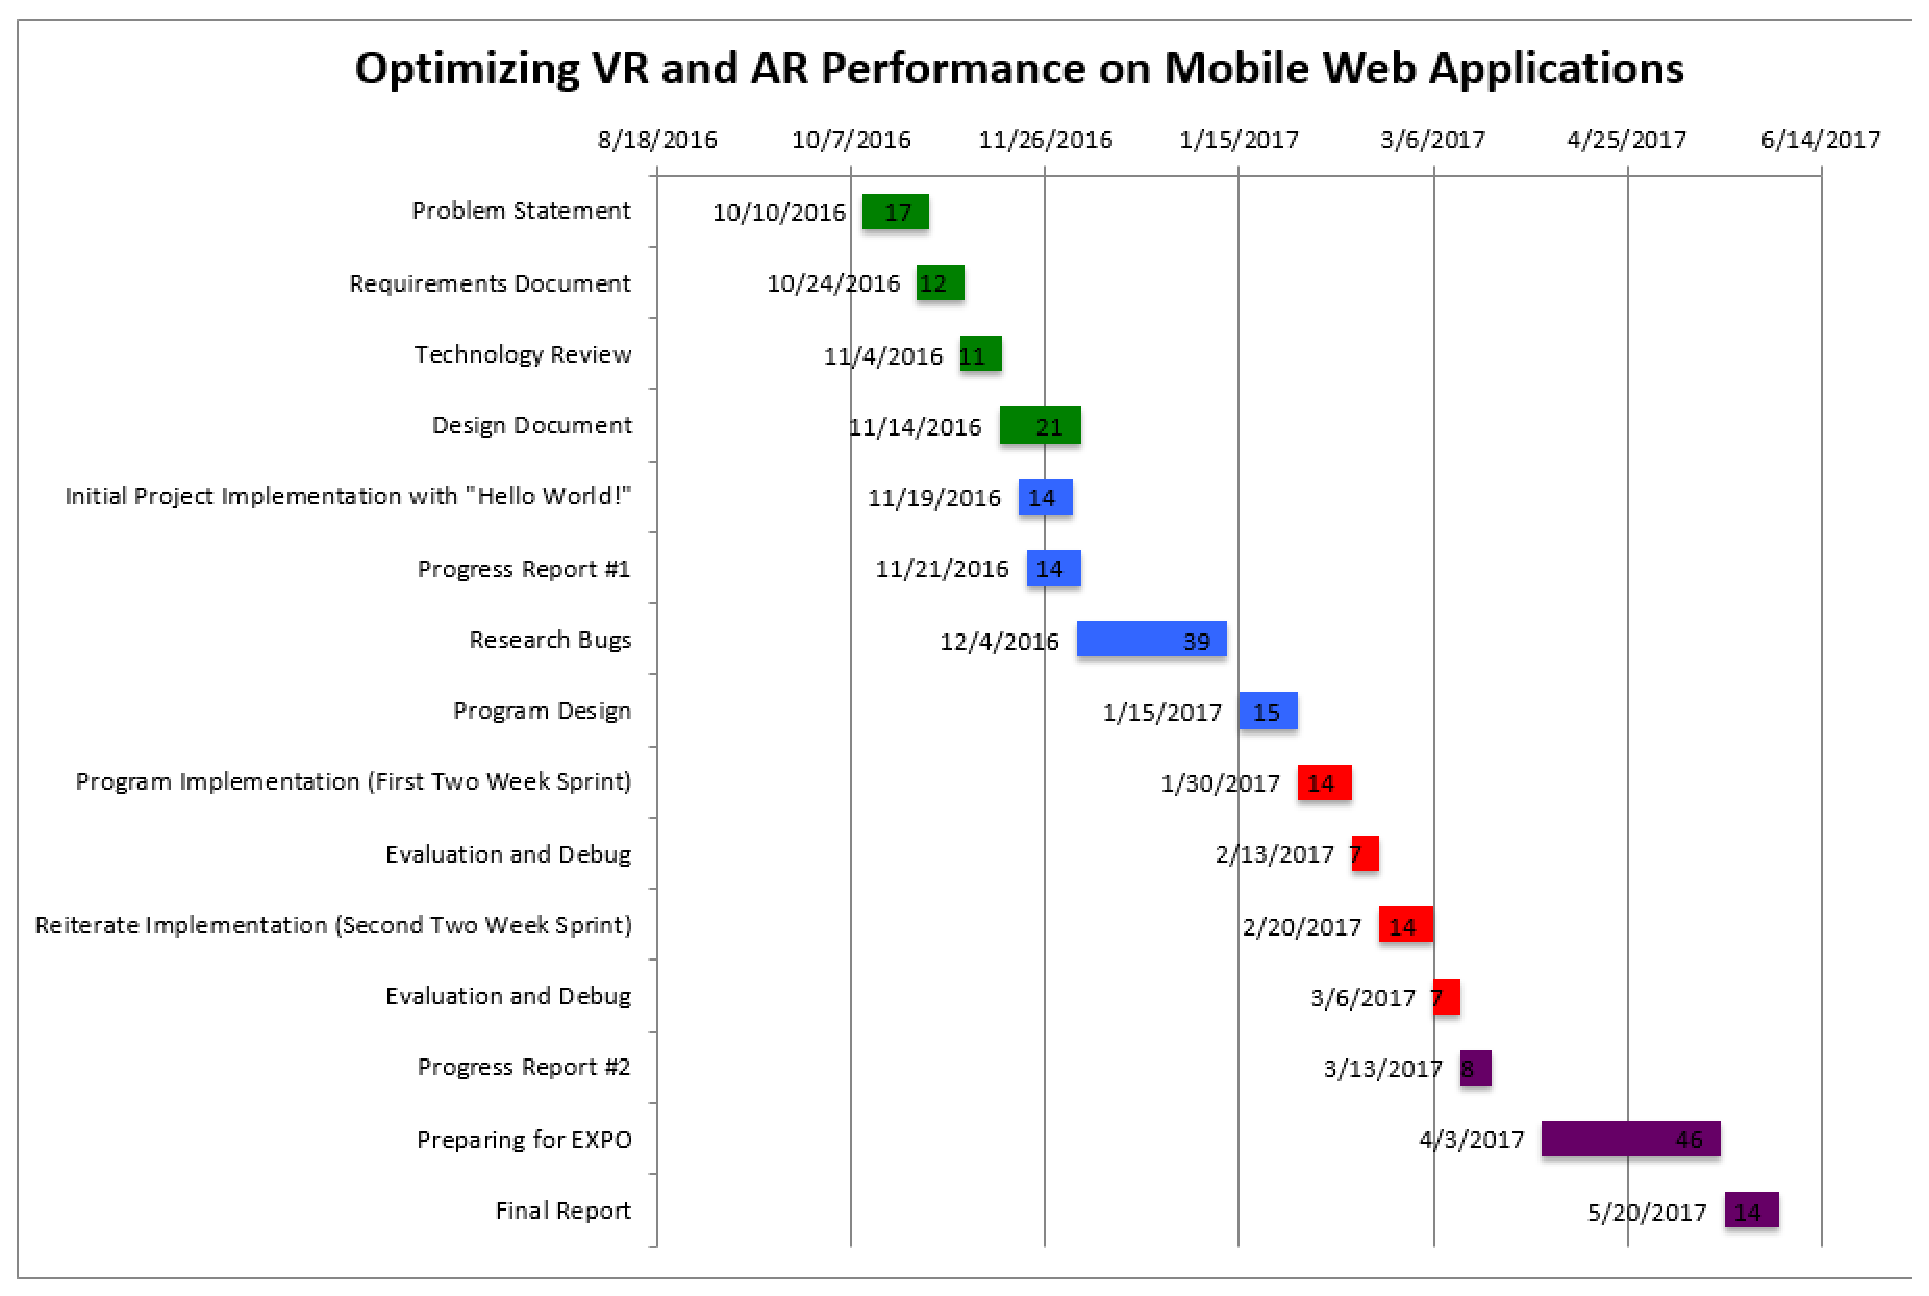
\includegraphics[width=1\textwidth]{OVRAR_Gantt_Chart.eps}
    \end{center}
\end{figure} 
\vfill

\begin{tabular}{ll}
\makebox[3.5in]{\hrulefill} & \makebox[1.5in]{\hrulefill}\\
Client Signature & Date\\
[4ex]% adds space between the two sets of signatures
\makebox[3.5in]{\hrulefill} & \makebox[1.5in]{\hrulefill}\\
Group Signature & Date\\
[4ex]% adds space between the two sets of signatures
\makebox[3.5in]{\hrulefill} & \makebox[1.5in]{\hrulefill}\\
Group Signature & Date\\
[4ex]% adds space between the two sets of signatures
\makebox[3.5in]{\hrulefill} & \makebox[1.5in]{\hrulefill}\\
Group Signature & Date\\
\end{tabular}
\end{document}